% Original author-supplied screenshots, copied unchanged from paper/.
% Use the MDPI full-page figure width to keep interface details legible.
\begin{figure*}[!t]
\begin{adjustwidth}{-\extralength}{0cm}
\centering
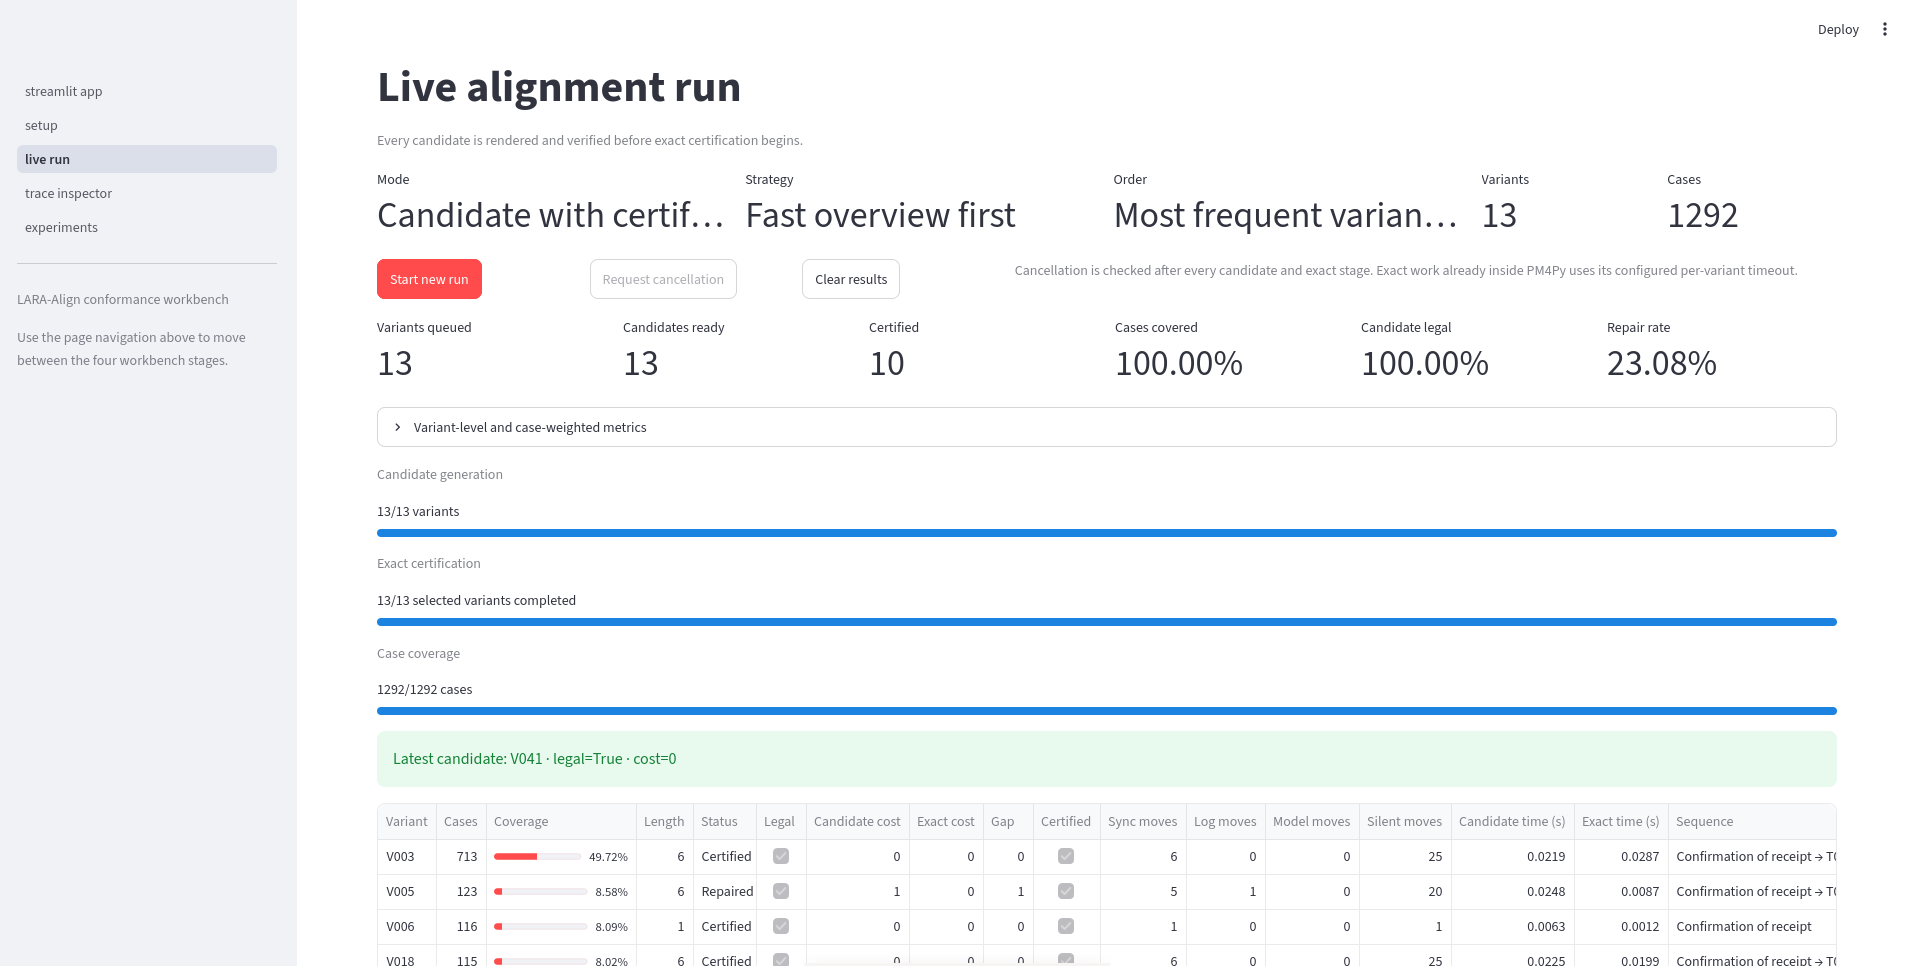
\includegraphics[width=\linewidth]{figures/lara-tool-live-run.png}
\end{adjustwidth}
\caption{The Live Run page of the LARA workbench. Progress indicators distinguish candidate generation, exact certification, and case coverage. The variant table keeps candidate legality, candidate and exact costs, gaps, certification status, and timings visible as separate fields. The displayed values describe the illustrated session.}
\label{fig:tool-live-run}
\end{figure*}

\begin{figure*}[!t]
\begin{adjustwidth}{-\extralength}{0cm}
\centering
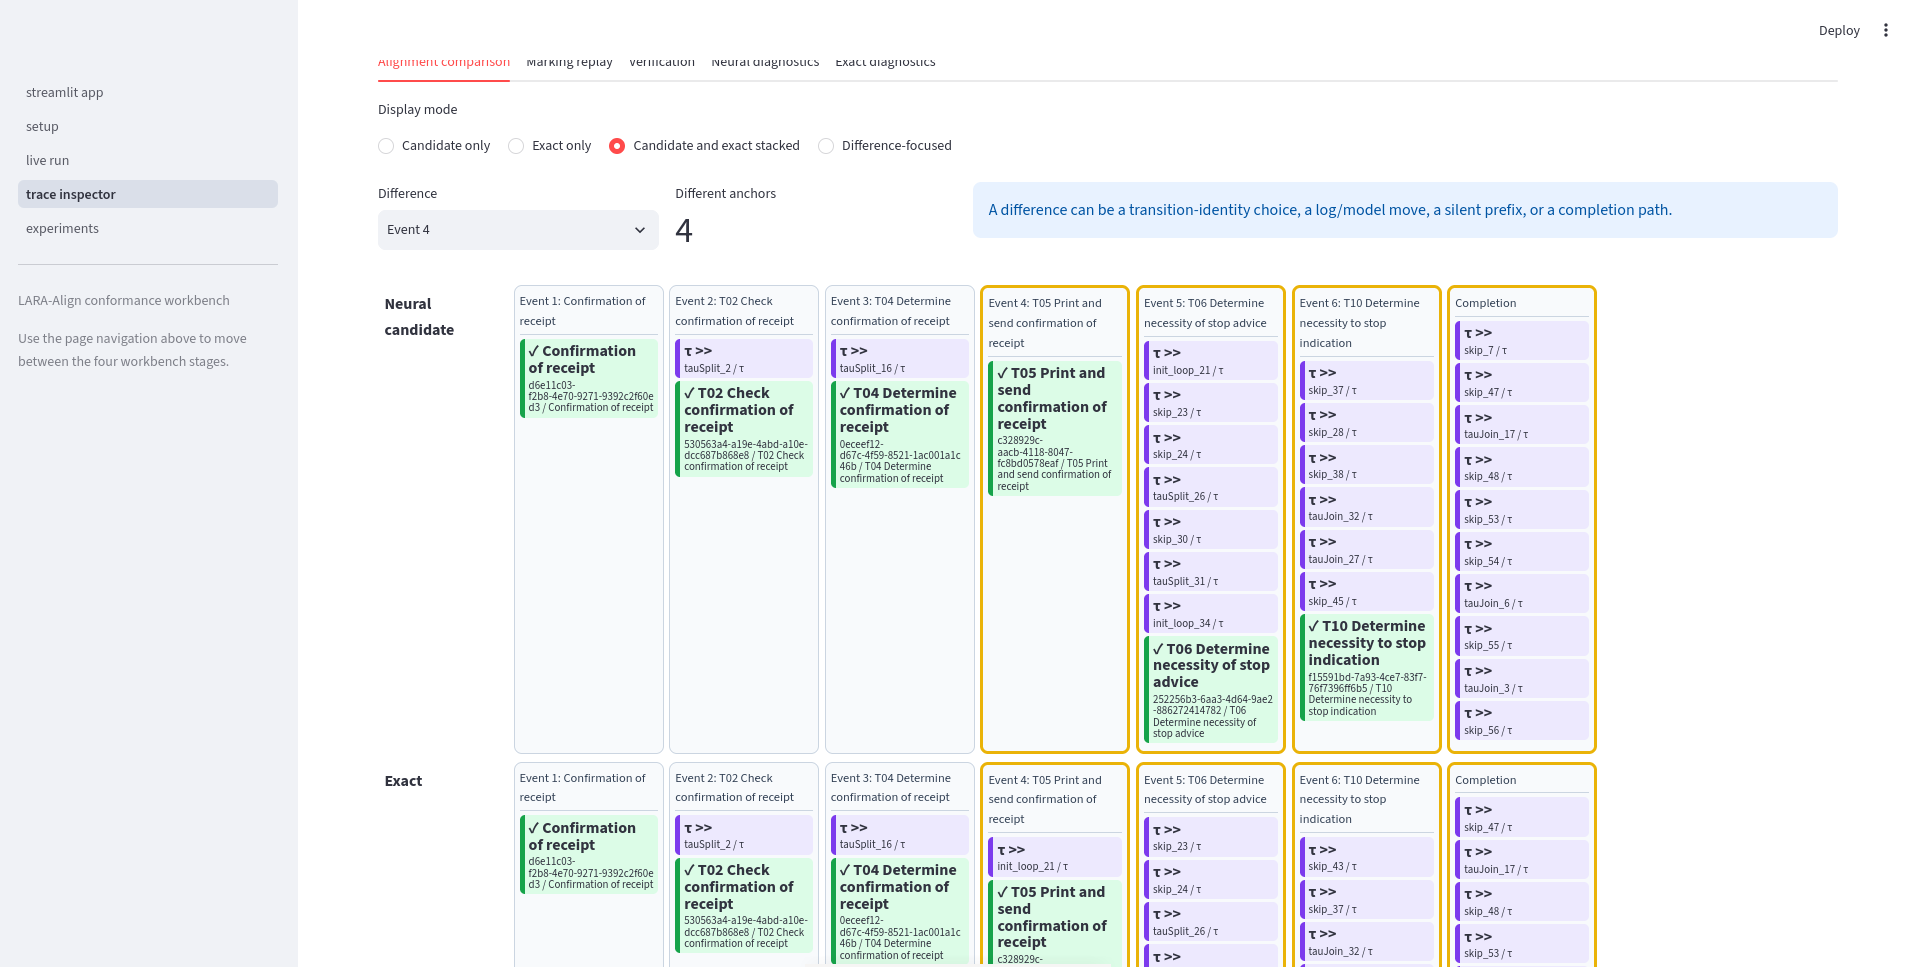
\includegraphics[width=\linewidth]{figures/lara-tool-trace-inspector.png}
\end{adjustwidth}
\caption{The Trace Inspector with candidate and exact alignments stacked at common event positions. Green cards show synchronous moves, purple cards show invisible model moves, and outlined columns mark differences between the explanations. Concrete transition identities and the separate completion column expose choices that a comparison of activity labels alone would hide.}
\label{fig:tool-trace-inspector}
\end{figure*}
